%% PROFE 2026 -- Matching subtask system description paper
%% CEUR-WS / IberLEF template (ceurart document class).
%%
%% HOW TO COMPILE
%%   This paper uses the official CEUR-WS class `ceurart.cls`.
%%   Easiest path: open this file in Overleaf and pick the
%%   "CEURART" template (Menu > Copy contents into that project),
%%   or download ceurart.cls + the CEUR bib style from
%%   https://github.com/yamadharma/ceurart and place them next to this file.
%%   Then: pdflatex main -> bibtex main -> pdflatex main -> pdflatex main
%%
%% >>> FILL IN THE PLACEHOLDERS MARKED WITH  %% TODO  BEFORE SUBMITTING <<<

\documentclass{ceurart}   % single-column CEUR-WS layout (as in ejemplo.pdf)

\usepackage{listings}
\usepackage{booktabs}
\usepackage{graphicx}

\lstset{
  basicstyle=\ttfamily\footnotesize,
  breaklines=true,
  columns=fullflexible,
  frame=single,
  framesep=4pt,
  xleftmargin=4pt,
  aboveskip=6pt,
  belowskip=6pt
}

\begin{document}

\copyrightyear{2026}
\copyrightclause{Copyright for this paper by its authors.
  Use permitted under Creative Commons License Attribution 4.0
  International (CC BY 4.0).}

\conference{IberLEF 2026, September 2026, [city], Spain} %% TODO: venue/city

%% TODO: replace with your real team name and title.
\title{[TEAM] at PROFE 2026: Text-Only Prompting of a Quantized
  Instruction-Tuned LLM for the Spanish Reading-Comprehension Matching Subtask}

%% TODO: author names, ORCID (optional), and email.
\author[1]{First Author}[
  email=davidbojaca1@gmail.com,
]
\author[1]{Second Author}[
  email=second.author@example.com,
]
\address[1]{[Affiliation / University], Spain} %% TODO

\begin{abstract}
  This paper describes our participation in the Matching subtask of
  PROFE~2026 (Spanish Language Proficiency Evaluation) at IberLEF~2026.
  The subtask reuses real Instituto Cervantes proficiency exams (levels
  A1--C2) and provides no task-specific training data, encouraging
  transfer-learning and generative Large Language Model (LLM) approaches.
  A novelty of this edition is that some exercises contain images that may
  or may not carry information needed to answer.
  We frame matching as a zero-shot, structured-output problem and solve it
  with a single open-weights instruction-tuned model,
  \texttt{Qwen2.5-7B-Instruct}, loaded in 4-bit precision so that the whole
  pipeline runs on a single 16\,GB GPU. The model receives a Spanish
  free-form reasoning prompt and emits a JSON object mapping every question
  to one option; a validated parser with fallbacks guarantees a well-formed
  submission. Our text-only system reaches \textbf{66.67\%} accuracy on the
  hidden test set, \textbf{+15.6} points over the official ChatGPT baseline
  (0.51). We additionally ran a controlled comparison against a multimodal
  variant (\texttt{Qwen2.5-VL-7B-Instruct}); contrary to intuition, naively
  feeding the images \emph{lowered} accuracy, because most images in this
  subtask are decorative rather than informative. Our main finding is that,
  for the matching subtask, a carefully prompted text-only model is a strong
  and resource-efficient baseline, and that visual information must be
  integrated selectively rather than indiscriminately.
\end{abstract}

\begin{keywords}
  Large Language Models \sep
  Prompting \sep
  Reading Comprehension \sep
  Spanish \sep
  Quantization \sep
  Multimodal reasoning \sep
  IberLEF
\end{keywords}

\maketitle

% =====================================================================
\section{Introduction}
% =====================================================================
Deep language comprehension---the ability to recover semantic nuances and
perform logical inference over a text---is a long-standing goal of Natural
Language Processing (NLP). A recurring obstacle in evaluating comprehension
is the construction of resources that genuinely test reasoning rather than
memorisation: many benchmarks are English-centric and contain training data
highly similar to the test set, which inflates apparent reasoning
ability~\cite{lai2017race}.

PROFE~2026~\cite{profe2026overview} addresses this by reusing Spanish
language-proficiency exams developed over many years by the Instituto
Cervantes to assess human students. Automatic systems are evaluated under
the same conditions as humans: they receive the exercises and their
instructions, with \emph{no} specific training material. This setup
deliberately favours transfer-learning and generative LLM approaches and
penalises systems that rely on data contamination. As a novelty, this
edition introduces exercises that contain images: some images are the
candidate answers, some provide information needed to answer, and some are
purely decorative. Systems must therefore decide \emph{when} visual cues are
relevant and when they should be ignored~\cite{penas2026profe}.

We participate in the \textbf{Matching subtask}, in which each exercise
provides two sets of items: systems must find, for every item in the second
set (the questions), the single item in the first set (the options) that
best corresponds to it. The first set may contain extra, unnecessary
options (distractors), and each option is used at most once.

Our work is guided by two research questions:
\begin{enumerate}
  \item Can an open-weights, instruction-tuned LLM, used purely
        zero-shot through prompting, solve the Spanish matching subtask
        clearly above the official baseline---while remaining cheap enough
        to run on a single consumer-grade GPU?
  \item Given that only a minority of exercises contain images and that many
        of those images are decorative, does adding a multimodal model
        help, or does indiscriminate visual input hurt?
\end{enumerate}

\noindent\textbf{Contributions.}
(i)~We present a reproducible, resource-efficient text-only pipeline built on
\texttt{Qwen2.5-7B-Instruct} in 4-bit precision that obtains
\textbf{66.67\%} accuracy on the hidden test set, \textbf{+15.6} points over
the ChatGPT baseline (0.51).
(ii)~We design a robust structured-output strategy---a Spanish free-form
reasoning prompt with a trailing JSON answer, a validated parser, and an
automatic detector of degenerate (constant-letter) outputs---that guarantees
a well-formed submission for every exercise.
(iii)~Through a controlled comparison we show that a multimodal variant
(\texttt{Qwen2.5-VL-7B-Instruct}) \emph{degrades} accuracy on this subtask,
providing concrete evidence that visual relevance must be filtered rather
than assumed.

% =====================================================================
\section{Related Work}
% =====================================================================
\textbf{Reading-comprehension benchmarks from human exams.}
Reusing human examinations to build comprehension benchmarks is an
established idea: RACE~\cite{lai2017race} derives multiple-choice questions
from English exams for middle- and high-school students. PROFE follows the
same philosophy but for Spanish, drawing on the IC-UNED-RC-ES corpus of real
Instituto Cervantes exams~\cite{penas2026profe}, which spans CEFR levels A1
to C2 and several exercise types (multiple choice, matching, and fill the
gap). Because the gold standard is not distributed, the benchmark is
resistant to contamination and to overfitting in post-campaign experiments.

\textbf{Large Language Models and prompting.}
Modern LLMs exhibit strong zero- and few-shot behaviour when steered through
natural-language prompts~\cite{brown2020gpt3,liu2021prompt,zhao2023survey}.
Eliciting intermediate reasoning---chain-of-thought
prompting~\cite{wei2022cot}---and aggregating multiple reasoning paths via
self-consistency~\cite{wang2023selfconsistency} are known to improve
performance on tasks that require multi-step inference. We adopt a free-form
reasoning prompt in Spanish and a structured (JSON) final answer, and we
experiment with self-consistency as an optional decoding strategy.

\textbf{Efficient inference and multimodality.}
We use the open-weights \texttt{Qwen2.5} family~\cite{qwen25} and its
vision-language counterpart \texttt{Qwen2.5-VL}~\cite{qwen25vl}. To fit a 7B
model and its activations within a single 16\,GB GPU, we rely on 4-bit
NF4 quantization in the style of QLoRA~\cite{dettmers2023qlora}, served
through the Hugging Face Transformers library~\cite{wolf2020transformers}.
Unlike QLoRA, however, we perform \emph{no} fine-tuning: the model is used
strictly in inference, consistent with the no-training-data spirit of the
task.

% =====================================================================
\section{Task and Dataset Description}
% =====================================================================
\textbf{The matching subtask.}
Each matching exercise contains a \emph{set~1} of option texts (identified by
letters, e.g.\ A, B, C, \dots) and a \emph{set~2} of question items
(identified by integers). The system must assign to every question the
single option that best matches it. There is exactly one correct option per
question, options are not reused, and set~1 may include extra options that
match no question. Some instructions explicitly warn about these
distractors (e.g.\ \textit{``HAY TRES TEXTOS QUE NO DEBE RELACIONAR''}).

\textbf{Statistics of the released test set.}
The matching test set comprises \textbf{189} exercises drawn from
\textbf{126} exams, with a total of \textbf{1{,}394} questions (matching
points). On average an exercise offers $8.88$ options (set~1, range 3--11)
for $7.38$ questions (set~2, range 6--10), so most exercises contain a small
number of distractor options. Exercises span the full CEFR range from A1 to
C2; Figure~\ref{fig:levels} shows their distribution. A1 and A2 dominate the
collection, while B2 and C1 are the rarest levels.

\begin{figure}[t]
  \centering
  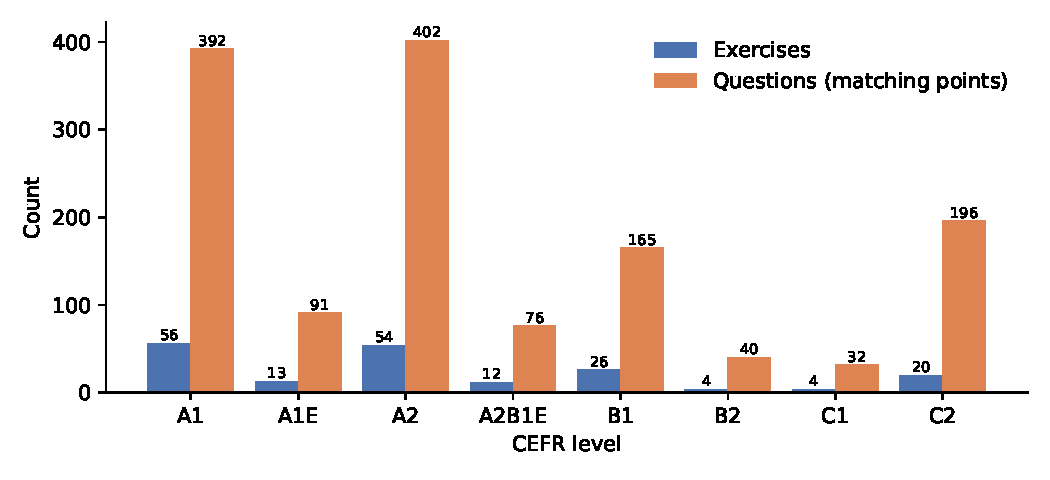
\includegraphics[width=\linewidth]{figures/level_distribution.pdf}
  \caption{Distribution of matching exercises and questions per CEFR level
    in the test set. Lower levels (A1/A2) dominate; B2 and C1 are scarce.}
  \label{fig:levels}
\end{figure}

\textbf{Images.}
Out of 189 exercises, \textbf{71 (37.6\%)} contain at least one image. Most
of these images appear on the \emph{question} side: there are 308 image
references in set~2 but only 81 in set~1, and only \textbf{27 exercises
(14.3\%)} have an image among the options. Manual inspection shows that a
large share of the question-side images are decorative (e.g.\ topic icons,
horoscope ornaments) rather than carriers of answer-relevant information.
This observation directly motivates our second research question and our
selective treatment of visual input (Section~\ref{sec:method}).

\textbf{Evaluation.}
The official metric is accuracy: the proportion of questions for which the
predicted option matches the gold option. This is the same measure applied
to human examinees, enabling a direct human--machine comparison. The
organisers report a preliminary baseline obtained with ChatGPT of
\textbf{0.51} for the matching subtask, which we adopt as our reference
point.

% =====================================================================
\section{Methodology}
\label{sec:method}
% =====================================================================
We frame matching as a single-shot, structured-prediction problem: for one
exercise, the model reads the instructions, all options, and all questions,
and produces a JSON object that maps each question identifier to an option
letter. No gradient updates are performed at any point; the system is purely
zero-shot. We justify each design decision below.

\subsection{Model and quantization}
We use \texttt{Qwen2.5-7B-Instruct}~\cite{qwen25}, an open-weights
instruction-tuned model with strong multilingual (including Spanish) and
instruction-following abilities. We chose a 7B model---rather than a larger
one---because the task constraints (free-tier Colab) cap available memory,
and because preliminary experiments with a 14B model did not improve over
the 7B configuration while being substantially slower. The model is loaded
in 4-bit NF4 precision with double quantization and a \texttt{bfloat16}
compute dtype~\cite{dettmers2023qlora}, which is what makes a 7B model fit
and run on a single 16\,GB GPU.

\subsection{Prompt design}
Each query consists of a system message that casts the model as an expert in
Spanish reading comprehension and instructs it to prefer literal, specific
matches over vague paraphrases, followed by a user message that lays out the
exercise. The user message lists the valid option identifiers, the option
texts, the question texts, and a strict instruction to reason briefly and
then output a single-line JSON object covering every question. The exact JSON
template (with the real identifiers of each exercise) is injected into the
prompt so the model knows precisely which keys and which letters are valid.
Listing~\ref{lst:prompt} shows the template.

\begin{lstlisting}[caption={Prompt template (system message and the skeleton
  of the user message). Curly-brace fields are filled per exercise.},
  label={lst:prompt}]
SYSTEM:
Eres un experto en comprension lectora del espanol, especializado en
examenes de proficiencia linguistica (Instituto Cervantes). Resuelves
ejercicios de tipo "matching" leyendo cuidadosamente cada texto y
eligiendo la mejor correspondencia. Prioriza coincidencias literales y
especificas sobre parafrasis vagas.

USER:
INSTRUCCIONES DEL EJERCICIO:
{instructions}

TEXTOS DEL SET 1 (identificadores validos: {set1_ids}):
{set1_block}

PREGUNTAS DEL SET 2 (identificadores: {set2_ids}):
{set2_block}

TAREA: Para cada pregunta del Set 2, decide que texto del Set 1 le
corresponde mejor. Razona brevemente y, al FINAL de tu respuesta,
escribe SOLO una linea con un JSON que asocie cada identificador del
Set 2 con un identificador del Set 1.

REGLAS ESTRICTAS:
- Cada respuesta DEBE ser una de estas letras: {set1_ids}.
- Nunca uses '-', 'ninguno' ni vacios. Si dudas, elige la opcion mas
  probable.

Formato exacto del JSON final (una sola linea, sin texto extra despues):
{"q1": "<letra>", "q2": "<letra>", ...}
\end{lstlisting}

For the text-only system, options or questions that consist of (or include)
an image are rendered with an explicit note stating that the element
contains an image that the model cannot see and that it should rely on the
surrounding text. This keeps the prompt honest about missing modality
instead of silently dropping the item.

\subsection{Decoding}
The submitted system uses \textbf{greedy decoding with a single sample}
(\mbox{$N=1$}) and a generation budget of up to 1{,}500 new tokens, which is
enough for short Spanish reasoning followed by the JSON line. We also
implemented self-consistency~\cite{wang2023selfconsistency} ($N=3$:
one greedy sample plus two sampled at temperature $0.4$, with a per-question
majority vote). Self-consistency roughly triples inference time; under the
free-tier time budget the single-sample greedy configuration was the one
used for the best official submission.

\subsection{Robust output parsing}
LLM free-form output is not guaranteed to be valid JSON, and an
ill-formed answer would forfeit an entire exercise. We therefore parse
defensively in three layers:
\begin{enumerate}
  \item \textbf{Validated JSON extraction.} We scan the generated text for
        JSON objects (last to first) and accept the first one that contains
        \emph{all} question identifiers; each value is upper-cased and kept
        only if it is a valid option letter for that exercise. This step
        rejects malformed answers and spurious values such as \texttt{"-"}
        or \texttt{"ninguno"}.
  \item \textbf{Regex fallback.} For any question still unresolved, we search
        the text near that question identifier for the first valid option
        letter.
  \item \textbf{Default fallback.} If both fail, we assign the first option
        letter so that every question receives an answer.
\end{enumerate}
After generation we additionally flag \emph{degenerate} exercises---those
where (almost) all questions received the same letter, a typical symptom of
the model refusing to answer and the parser repeatedly hitting the default
fallback---and re-run them. Three exercises were detected and re-run this
way.

\subsection{Multimodal variant (ablation)}
To answer the second research question we built a parallel pipeline with
\texttt{Qwen2.5-VL-7B-Instruct}~\cite{qwen25vl}, also in 4-bit precision. The
prompt structure is identical, but real images are passed to the model
instead of the ``cannot see'' note. To control memory, each image is
down-scaled so that its longest side is at most 512 pixels, generation is
capped at 600 tokens, and out-of-memory exercises fall back to the text-only
prediction. We applied this variant only to the exercises that contain
images and compared it against the text-only predictions.

\subsection{Reproducibility}
\label{sec:repro}
All experiments ran in Google Colab on a single \textbf{NVIDIA T4
(16\,GB)} GPU under the free tier. The model is
\texttt{Qwen2.5-7B-Instruct} served with Hugging Face
Transformers~\cite{wolf2020transformers} and \texttt{bitsandbytes} 4-bit
NF4 quantization (double quantization, \texttt{bfloat16} compute). Decoding
is greedy ($N=1$), \texttt{max\_new\_tokens}=1500. Predictions are written
incrementally (one exercise at a time) so that long runs can be interrupted
and resumed without losing work. The submission is a JSON file mapping each
\texttt{exerciseID} to a \{question: option\} dictionary. The code (a single
Colab notebook) is available at:
\begin{center}
  \url{https://github.com/<your-username>/profe2026-matching} %% TODO
\end{center}

% =====================================================================
\section{Results}
% =====================================================================
Table~\ref{tab:results} reports accuracy on the hidden test set. Our
text-only system reaches \textbf{66.67\%}, clearly surpassing the official
ChatGPT baseline of 0.51 by \textbf{15.6} points. The multimodal variant did
\emph{not} improve over the text-only system; on the contrary, replacing
text-only predictions with multimodal ones on the image-bearing exercises
\emph{reduced} overall accuracy.

\begin{table}[t]
  \centering
  \caption{Accuracy on the PROFE~2026 matching test set (question level).
    The text-only system is our official submission.}
  \label{tab:results}
  \begin{tabular}{lc}
    \toprule
    \textbf{System} & \textbf{Accuracy} \\
    \midrule
    ChatGPT baseline (organisers) & 0.5100 \\
    \textbf{Ours --- Qwen2.5-7B-Instruct, text-only ($N{=}1$)} & \textbf{0.6667} \\
    Ours --- Qwen2.5-VL-7B, multimodal on image exercises & $<0.6667$\,$^{\dagger}$ \\
    \bottomrule
  \end{tabular}

  \vspace{2pt}
  {\footnotesize $^{\dagger}$ The multimodal variant scored below the
   text-only system; %% TODO: insert the exact Codabench score here.
   see Section~\ref{sec:errors} for the analysis.}
\end{table}

On the small set of labelled \emph{example} exercises released by the
organisers (27 questions across three exercises---the only matching data
with a public gold standard), the text-only system answered 24 correctly
(88.9\%).
%% TODO: confirm this 24/27 figure; it was our observed dev result.
This is consistent with the test-set result being lower, since the hidden
set is larger and includes harder, higher-level (C1/C2) exercises that are
absent from the examples.

% =====================================================================
\section{Error Analysis}
\label{sec:errors}
% =====================================================================
Because the organisers do not release the test gold standard, our error
analysis combines (a) the labelled example exercises, (b) the structure of
the model's raw outputs, and (c) the controlled text-only vs.\ multimodal
comparison.

\textbf{Structured-output failures.} Early runs occasionally produced
invalid answer tokens (e.g.\ a literal \texttt{"-"}) or refused to commit to
a letter. These never reach the submission thanks to the validated parser,
but they reveal that the model is uncertain on some items. The
degenerate-output detector flagged three exercises in which nearly all
questions collapsed to a single letter; re-running them produced
better-differentiated answers.

\textbf{Distractors.} The hardest configurations are exercises with several
extra options (set~1 larger than set~2), and especially the 13 exercises
that explicitly contain options that must \emph{not} be matched. Here the
model must not only find the best option but also avoid being attracted by a
plausible but unused distractor; this is where literal-match prompting
(``prefer literal, specific matches over vague paraphrases'') helps most.

\textbf{Paraphrase vs.\ literal matching.} Qualitatively, correct matches
tend to hinge on a specific lexical or factual anchor shared between question
and option (a name, a number, a concrete fact), whereas errors cluster on
questions phrased as broad paraphrases of a whole text, where two options are
semantically close.

\textbf{Why multimodality hurt.} The multimodal variant lowered accuracy for
three compounding reasons. First, most images are on the \emph{question} side
and are decorative (icons/ornaments); feeding them adds distracting tokens
without adding signal. Second, our 512-pixel down-scaling, needed to fit the
vision model in memory, degrades any text embedded in an image, so even the
genuinely informative images are read poorly. Third, and most importantly,
the variant \emph{overwrote} text-only predictions on the image-bearing
exercises---many of which the text-only model had already answered correctly
using the option texts alone---trading correct answers for noisier ones. The
lesson is that visual input on this subtask must be \emph{gated} by an
estimate of visual relevance, not applied indiscriminately.

% =====================================================================
\section{Conclusion and Future Work}
% =====================================================================
We described our system for the Matching subtask of PROFE~2026. A single
open-weights, instruction-tuned model (\texttt{Qwen2.5-7B-Instruct}), used
zero-shot in 4-bit precision with a Spanish free-form reasoning prompt and a
validated JSON output, reaches \textbf{66.67\%} accuracy on the hidden test
set, \textbf{+15.6} points over the official ChatGPT baseline, while running
on a single free-tier 16\,GB GPU. This answers our first research question
affirmatively: careful prompting of a modest, quantized LLM is a strong and
cheap approach to Spanish reading-comprehension matching.

Our second finding is a cautionary one. A multimodal model did not help and
in fact hurt, because the majority of images in this subtask are decorative
and because indiscriminately replacing text-only answers discards good
predictions. This validates the task organisers' premise that systems must
\emph{discern when to integrate visual cues and when to disregard them}.

\textbf{Future work.} The natural next step is a visual-relevance gate: a
cheap classifier (or a prompt-based judgement) that decides, per exercise,
whether an image is informative before invoking the vision model, so that
multimodal reasoning is applied only where it can help. Other promising
directions are OCR or higher-resolution encoding for images that contain
text, self-consistency or small ensembles within a larger time budget, and
exploiting the publicly available PROFE~2025 exams as in-context examples or
for light fine-tuning of the option-selection behaviour.

% =====================================================================
\section*{Declaration on Generative AI}
% =====================================================================
During the preparation of this work, the authors used a generative AI
assistant in order to: draft and refine the experimental pipeline, format
results, and perform grammar and spelling checks. After using these tools,
the authors reviewed and edited the content as needed and take full
responsibility for the publication's content.

\bibliography{refs}

\end{document}
